%TEX root = ../thesis.tex
%*******************************************************************************
%****************************** Second Chapter *********************************
%*******************************************************************************

\chapter{Methodology}

\ifpdf
\graphicspath{{Chapter2/Figs/Raster/}{Chapter2/Figs/PDF/}{Chapter2/Figs/}}
\else
\graphicspath{{Chapter2/Figs/Vector/}{Chapter2/Figs/}}
\fi

\section[Raw data]{Data consists of \textit{in vivo} confocal timelapses}
The majority of data used in this report is directly acquiried from Willis et
al.~\cite{willis2016cell}, and thus largely follows their approach for data
acquisition and processing. An introductory description is nevertheless outlined
below. 

Six plants, labelled plant 1, 2, 4, 13, 15, and 18, were grown on a
solution consisting of 10$\mu M$ auxin transport inhibitor NPA to a depth of
roughly 1~cm for 22-26 days. The inhibition of auxin prevents formation of new
primordia, and this gives rise to a small and naked, organ-free meristem which is
tractable for imaging. 

The plantlets were marked with pUBQ10::acyl-YFP, which localises in the cell
membrane, as well as with pCLV3::dsRED-N7, which was used
as a nuclear tracker for CLV3 mRNA expression. Also pPin1::PIN1-GFP was tracked,
but not quantified in this study. In addition, plant 1 did not express the nuclear marker
for CLV3, whereas plant 18 did not undergo successful nuclear segmentation. Both
are therefore completely excluded from the nuclear analysis.

Using confocal microscopy, the six plantlings were tracked in
intervals of 4 hours up to 76 (plants 1, 2 and 4) or 84 hours
(plants 13, 15 and 18), using a 63x/1.0 N.A.\ water immersion objective.
Due to the high resolution of the images, the acquisition of each z-stack took
$\sim$10 minutes, which caused vertical stretching in the images due to stem
elongation. Because of this, a second batch of z-stacks was acquired, using
low-resolution imaging over $\sim$10 seconds. The original images were then
corrected, using this second batch as reference.

\begin{figure}[H]
  \centering
  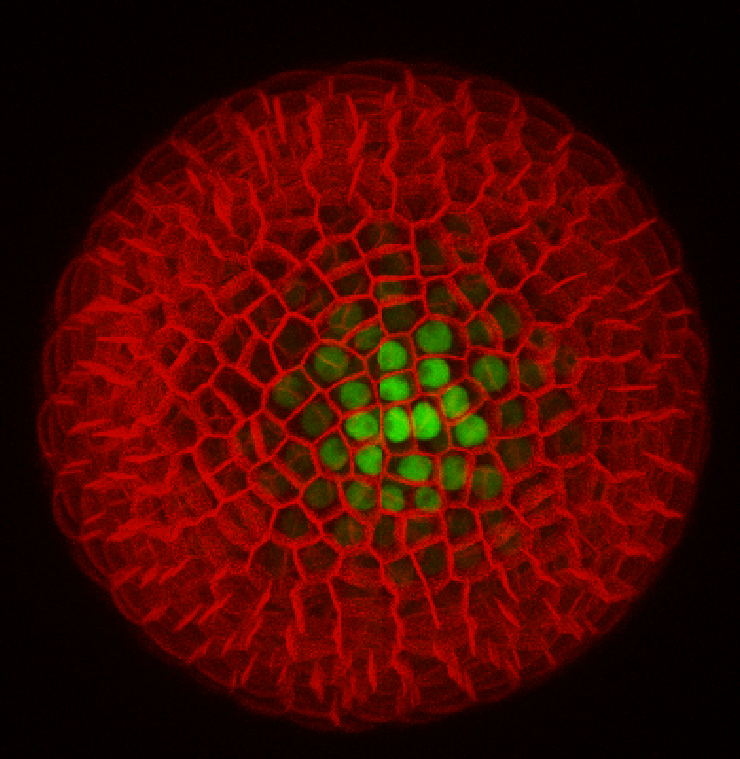
\includegraphics[width=.4\textwidth]{raw_channels.png}
  \caption[Confocal microscopy data]{Topview of raw data as produced by the
    confocal imaging, taken from plant 2 at timepoint 0 hours. In red can be
    seen the membrane channel, merged with the
    nuclear response in green. The nuclear vacuole is observable as shaded dots
    in the green channel. Note also how the L2 and L3 produce a percieved
    fuzziness in the peripheral regions.}
  \label{fig:rawdata}
\end{figure}

\section[Processed image data]{Image pre-processing and segmentation}
In order to eliminate segmentation errors, the ImageJ plugin StackReg was used
to perform a translation transformation for each stack. Individual slices which
contained horizontal shifts because of vibrations or other types of system
disturbances were identified and replaced with the nearest slice that contained
no such shift. The z-directional stretching due to stem elongation was corrected for by mapping
the low-resolution stacks to the high-resolution ones in order to attain
stretching factors that the images were thereafter corrected for. 

For the membrane channel, noise removal was done by Gaussian and alternative-sequential
filtering. The filtered z-stacks were then watershed in 3D using the
algorithm implemented in the segmentation software MARS-ALT (see
\cref{sec:software_descr}). Segmentation and
tracking was thereafter performed using the same software. Cellular volumes were from
this then calculated as the sum of voxel volumes belonging to the same cell.
The tracking, also performed using MARS-ALT, was assessed for quality using an F1
score between the parent and corresponding daughter cell. For all analyses
discussed in this report, a cutoff value of 0.30 was set for the tracking in
order to account for incorrect mappings. These cells are included in the
overall analysis, but excluded from all cell line related investigations.
A longer outline of errors and exceptions in the segmentation is presented in
\cref{sec:data_errors}.   

The nuclear data were deconvolved to account for the microscope's point-spread
function using the \textit{PSF distiller} tool from Huygens software 15.05. As
in the membrane case, the nuclear channels were adjusted with the  
corresponding stretching factors and thereafter segmented using segmentation
tool Costanza~\cite{costanza} (see \cref{sec:costanza}). Whenever we in this
thesis mention the CLV3 expression, we refer to the mean fluorescence of the
voxels belonging to the corresponding nucleus. 

\begin{figure}[H]
    \centering
    \begin{minipage}{0.49\textwidth}
        \centering
        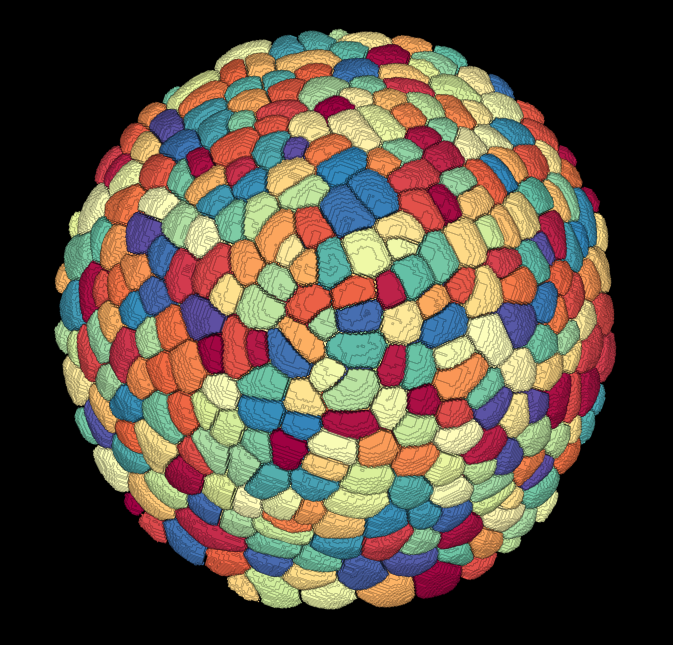
\includegraphics[width=.95\textwidth]{plant18_t0.png}
      \end{minipage}\hfill
      \begin{minipage}{.49\textwidth}
        \centering
        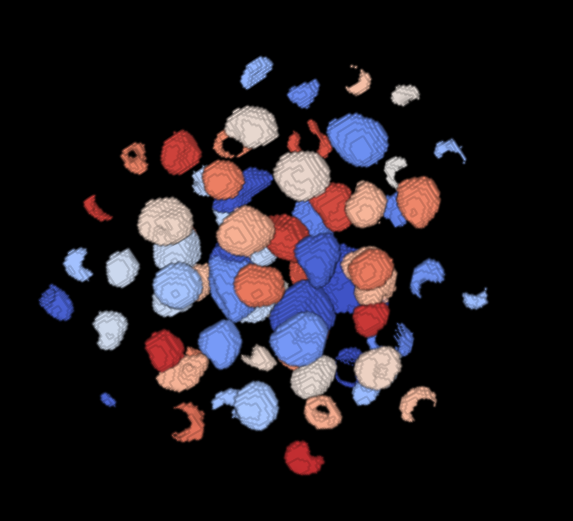
\includegraphics[width=\textwidth]{plant18_t0_n.png}
      \end{minipage}
      \caption[Segmented data]{Segmented membrane and nuclear channels as output by
        visualisation software TissueViewer after MARS-ALT and
        Costanza segmentation respectively (see \cref{sec:software_descr}). Note in the nuclear channel
        how the loss of signal due to the vacuole causes missegmentation in
        multiple cases. Figures taken from plant 18, timepoint 0 hours. Nuclear
        and membrane channels not to scale.}  
\end{figure}

% Nuclear and membrane mapping
Due to the membrane and nuclear segmentations originating from different
softwares, a separate mapping step was required in order to relate nuclei to
their corresponding cell membranes. This was done by taking the centroid spatial
coordinates, as defined by the basins of attraction acquired during
segmentation, of all respective segmented items, and mapping them using a
least-squares approach. Duplicately mapping nuclei were then
consolidated as described in \cref{sec:filtering}. 

% Distance measures (d2t / circ)
Measures of distances to the top were done in multiple ways. The four methods
herein considered consist of a definition of the top based on 1) the spatial
coordinates, 2) the expression value, 3) expression-weighted spatial
coordinates, and 4) a least-square fit of a paraboloid to raw meristem images.
For the paraboloid fit, this is done by taking the top 75 images part of the
confocal z-stack, in order to minimise the fitting impact of primordia that
are more prominent in the deeper levels.
In the case of spatial coordinates, the average $x-y$  
coordinates of $n$ nuclei were chosen, complemented with the highest $z$ value
registered in the corresponding timeframe. For the second case, the apex was
defined as the mean spatial coordinates of the $n$ highest expressing CLV3
nuclei. The weighted apices were similarly determined through transformation via
$\bar{x}_{w} = \sum^{n}_{i} \bar{x}_{i}I_i / \sum_{i} I_i$, where $n$ again denotes number of cells included,
arranged by highest z-value, and $I$ the CLV3 intensity for the
corresponding cell.
Lastly, the parabloid fit to the meristem was used to define the apex by
taking the coordinates of the region have a zero-valued derivative. For both the
segmentation-dependent approaches, the data was set to exclude subepidermal
layers in order to prevent biases. 

To achieve a cell-resolution description of distances in the SAM,
an auxilliary measure of cell distances was used in the form of a cell-wise
grouping. In the cell value utilising definitions of the apex above, cells
included in the definition was set to have a cell-wise distance of 0. The
neighbours of these cells were in turn defined to have a distance value of 1,
and so on recursively. Again, we exclude the plants lacking nuclear data from
measures utilising this. In addition, whenever cells deeper in the tissue than L2 are
referenced, we refer to these as L3 and L3$+$ interchangeably.

\section[Data processing]{Data processing}
\label{sec:data_processing}
\subsection[Data analysis tools]{Development of a data analysis pipeline}
\label{sec:pipeline}
Data was analysed predominantly using R through the development of a single
modular pipeline, denoted \textit{extractoR}. This was designed to build 
primarily on a sequential software design pattern,  
incorporating parallelisation and batch processing for treatment of the multiple
timelapses. A more descriptive explanation is outlined in~\cref{extractoR}.

\subsection[Data filtering]{Data filtering}
\label{sec:filtering}
Due to thresholding effects for cell nuclei during the segmentation, some
individual nuclei are occasionally identified as two or more. Nuclei were
therefore mapped to the corresponding membranes using a minimum euclidian distance
measure between the respective centroids. The nuclear quantified metrics were
then corrected using the functions found in \cref{tab:consolidation_methods}. In
addition to this, all mentions of numbers of nuclei are with respect to the
number of cell membranes containing at least one nuclear volume identified
within them.

For the data analysis section, data was excluded due to apparent segmentation
errors. This was done for each plant in isolation, with the outline of the
filtering described in \cref{tab:filtering}. The choice of allowed
deviance was done based on the distribution shape, (TODO: Put these in appendix)
with particular consideration 
taken to the nuclear and membrane volumes, where no lower boundary was set. The
maximal neighbour distance was chosen due to the typical lack of data for cells more
than $7$ cell distances from the apex. Lastly, due to division events where
loss of nuclear signal took place, we filter out expression values which are
less than 70~\% of the magnitude in the previous, as well as subsequent timepoint.

\begin{table}
  \parbox{.47\linewidth}{
    \centering
    \begin{tabular}{ll}                            \toprule
      \textbf{Parameter} & \textbf{Value}       \\ \midrule
      Maximal membrane volume & $\mu + 3\sigma$ \\
      Minimal membrane volume & 0               \\
      Maximal nuclear volume  & $\mu + 5\sigma$ \\
      Minimal nuclear volume  & 0               \\
      Maximal apical distance & $\mu + 3\sigma$ \\
      Maximal neighbour distance & $7$          \\ \bottomrule   
      \vspace{.1em}
    \end{tabular}
    \caption[Filtering settings]{Filtering settings in order to account for outliers in the data.
      Typical causes of these are missegmentation such as the merging of multiple
      nuclear membranes of nuclei. Because the quaility declines with the distance to the
      apex we here limit our analysis to cases where cells are within a distance
      of 7 cells from the defined apex.}
    \label{tab:filtering}
  }
  \hfill
  \parbox{.47\linewidth}{
    \centering
    \begin{tabular}{lc}                                 \\ \toprule
      \textbf{Metric}       & \textbf{Summary function} \\ \midrule
      Coordinates (x, y, z) & mean                      \\
      Nuclear volume        & sum                       \\ 
      Nuclear expression    & mean                      \\ \bottomrule
      \vspace{.1em}
    \end{tabular}
    \caption[Consolidation methods for duplicate nuclei]{Consolidation methods applied for cases where multiple nuclei were
      mapped as belonging to the same membrane cell. This happens mainly due to
      errors  when one nuclei is identified as multiple in the
      binarisation step of the segmentation.}
    \label{tab:consolidation_methods}
  }
\end{table}

\section[Models of Gene Regulatory Networks]{Models of Gene Regulatory Networks}
\label{sec:models_of_grns}
\subsection[Mathematical Formulation]{Mathematical Formulation of Biochemical
  Reactions}
\label{sec:mathematical_form}

\subsubsection[Mass-action Kinetics]{Mass-action Kinetics}
\label{sec:mass_action}
The formulation of processes in GRNs focus primarily on two aspects: synthesis
and degradation of matter, which usually takes the form of molecular
concentrations or absolute abundance. As outlined in \cref{sec:modelling}, we
here work using an ODE or SDE description of  
our regulatory systems. 

In this study, we represent our molecular reactions using mass-action
interactions and Michaelis-Menten kinetics; both here relying on the na\"ive
assumption that our primary reagents here act in isolation of other possibly
intervening molecules. As part of our formalism, we write
\begin{equation}
  S \xrightleftharpoons[k_{f}]{k_{b}} P
  \label{eq:simple_reac}
\end{equation}
to express that some substrate $S$ is turned into a product $P$ by some given
\textit{forward affinity} $k_f$. Likewise, as the reaction is \textit{reversible}, the
product $P$ is transformed back into $S$ with the \textit{backward affinity}
$k_b$. 

The \textit{law of mass action} states that the rate of a reaction
is proportional to its affinity, e.g.\ $k_f$, and the concentration of the
reacting species, here $S$. The reaction rate of the production of $P$ would thus be
$r_f = k_f S$. However, the rate of change of reactant $P$ also depends
on the backward affinity, which would give the overall rate-of-change for $P$ as
\begin{equation}
  \Delta P = k_f S - k_b P.
  \label{eq:mass_action_noninf}
\end{equation}
In the infinitesimal limit, we analogously have 
\begin{equation}
  \frac{\dd P}{\dd t} = k_f S - k_b P,
  \label{eq:mass_action_inf}
\end{equation}
i.e.\ on the form of a differential equation, which will be the baseline for our
formulations. Similar to the formulation of a rate-of-change of $P$, we can do the
same for species $S$, and our system is then fully represented as a system of
differential equations.

Expanding on this, we can easily solve for the steady-state concentrations of
the system by assming that all rates average to zero. In our example above, this
gives us 
\begin{equation}
  \frac{k_f}{k_b} = \frac{P}{S},
  \label{eq:mass_action_ss}
\end{equation}
which holds in general, regardless of the number of reacting species.

\subsubsection[Michaelis-Menten Kinetics]{Michaelis-Menten Kinetics}
\label{sec:mm}
A conceptual drawback of the mass-kinetics formulation is the possibility to
have infinite reaction rates, whereas the molecular reactions in nature typically
are restricted by some means. One way to account for this is through
\textit{Michaelis-Menten kinetics}, which describes enzymatic chemical
reactions. In these, the trivial example introduced in \cref{eq:simple_reac} is
expanded to include an enzymatic agent such that
\begin{equation}
  E + S \xrightleftharpoons[k_f]{k_b} ES \xrightarrow{k_p} E + P.
  \label{eq:enzymatic_react}
\end{equation}
In other words, an enzyme-like molecule binds to the substrate $S$ such that the
complex $ES$ is formed. This complex is thereafter transformed into the product
molecule $P$ and again the enzyme $E$. Assuming a total enzyme concentration of
$E_{tot}$ and the assumption that the enzyme-substrate binding process is in
equilibrium, the rate-of-change of the product can be rephrased to be on the
form 
\begin{equation}
  \frac{\dd P}{\dd t} = V_{max} \frac{S}{K + S},
  \label{eq:michaelis-menten}
\end{equation}
where $K = K_f / K_b$ and $V_{max} = k_pE_{tot}$. This expression is said to be
on \textit{Michaelis-Menten} form, where $V_{max}$ is the maximal
activation rate of the protein, and $K$ can be thought of as a saturation
coefficient.

Extrapolating on this type of reaction, introducing $n$ enzymatically acting
molecules instad gives the standard \textit{Hill equation} form, namely
\begin{align}
  \frac{\dd P}{\dd t} &= V_{max} \frac{S^n}{K^n + S^n},\hspace{.8em} \text{and} \\
  \frac{\dd P}{\dd t} &= V_{max} \frac{K^n}{K^n + S^n}
  \label{eq:hill}
\end{align}
for an activating and repressing reaction respectively.

\subsection[Stochastic Simulations]{Numerically solving stochastic systems}
\label{sec:stoch_sim}
\subsubsection{Gillespie Algorithm}
\label{sec:gillespie}
The Gillespie algorithm is a discrete approach for simulating stochastic
molecular dynamics. It first appeared in print by Dan Gillespie in 1977, and has
since been widely used for stochastic simulations in multiple fields.

While being computationally expensive, the Gillespie algorithm compensates for
its lack in tractability by producing a statistically exact trace of the
molecular dynamics of a system. 

The algorithm originates in the formulation of the \textit{chemical master equation},
which specifies the rate of change of the transition probabilty between states
in the form of 
\begin{equation}
  \dfrac{\partial P\left( x,t | x_0, t_0 \right)}{\partial t} = 
  \sum_{j =
    1}^{M} \left[ a_j\left( x-v_j \right)P\left( x-v_j, t|x_0,t_0 \right) -
    a_j(x)P\left( x,t|x_0,t_0 \right) \right]
\end{equation}
where $a$ defines to reaction probability, or propensity, for each type of reaction, and
$v$ the stoichiometry, i.e. information of how the molecular species are changed
due to the reaction. $P(x,t | x_0, t_0)$ on its own denotes the probability of
$X(t) = x$, given that the initial value is $x_0$. Solving the master equation
analytically is usually complicated, so  
simulating a complex biological system using the Gillespie approach can often be
far more tractable.

Proceduraly, the algorithm can be formulated in four steps: 
\begin{description}
  \item[Initialisation] Generation of number of molecules and reaction
    parameters. 
  \item[Randomisation] Generation of random numbers to determine 1) next
    interaction, and 2) the time increment.
  \item[System update] Time and molecular numbers are update correspondingly
    to the determined event in step 2.
  \item[Repetition] Step 2-4 are repeated until some stop condition is met.
\end{description}

In principle, the Gillespie algorithm is interested in two fundamental
questions: 1) When does the next reaction happen? 2) Which is the next reaction?
The time until the next reaction at time $t$ is denoted $\tau$ and can be shown
to be an exponential distribution centered  
at $1 / \sum_{j=1}^{M}a_j(x)$ for some molecular concentration $x$, i.e.
\begin{equation}
  p(\tau = t') = \sum_{j=1}^M a_j(x)e^{-\sum_{j=1}^M a_j(x)t'}
  \label{eq:gill:time}
\end{equation}
with the reaction probability instead being described by the normalised
propensity. Historically, due to the limitation of random number generators, the
time update has been described as being drawn from 
\begin{equation} 
  \displaystyle
  \tau = \dfrac{1}{\sum_{j=1}^M a_j(x)} \ln\dfrac{1}{r_1}
  \label{eq:gill_time_update}
\end{equation}
with $r_1$ denoting a uniformly distribution random number in the interval
$(0,1]$.

\subsubsection{Milstein's Method}
\label{sec:milstein}
If there is no requirement for exactness, less computationally intense
alternatives to Gillespie's algorithm exists. One such example is the
\textit{Langevin} formulation of chemical systems, which utilises SDEs to
attain an approximate solution to the system trajectory, and is particularly
useful when the number of molecular reagents is high. 

The Langevin formulation, like Gillespie's, utilises the chemical master
equation to compute the behaviour of the system. In principle, the Langevin
formulation can be said to reformulate a deterministic increment of the form
\begin{equation}
  X_i(t + \dd{t}) = X_{i}(t) + \sum_{j=1}^M
  v_{ji}a_j(X(t))\dd{t}
  \label{eq:deterministic}
\end{equation}
to the stochastic form
\begin{equation}
  X_i(t + \dd{t}) = X_{i}(t) + \sum_{j=1}^M
  v_{ji}a_j(X(t))\dd{t} + \sum_{j=1}^M
  v_{ji}a_j^{1/2}N_j(t)\dd{t}^{1/2}
  \label{eq:stoch}
\end{equation}
where $X$ denotes the molecular number, $v$ the stochiometric coefficient of the
equation in question, and $N_j$ are temporally uncorrelated and statistically
independent, Gaussian random numbers with mean 0. From this stage, the equation
is then easily extended to its multivariate form, namely
\begin{equation}
  X_i(t + \dd{t}) = \sum_{j=1}^Mv_{ji}a_j(\bar x) \dd{t} +
  \sum_{j=1}^M v_{ji}{a_j}^{1/2}(\bar x) N_j(t) \left( \dd t \right)^{1/2}
  \label{eq:stoch_multi}
\end{equation}

Milstein's approach to solving this equation numerically utilises
\cref{eq:stoch} on the differential form 
\begin{equation}
  \dd X_t = a(X_t) + b(X_t) \dd W_t
  \label{eq:milstein_form}
\end{equation}
where $W_t$ is a continuous-time stochastic process. The simulation interval
$\left[ t_0, T \right]$is then partitioned into parts of size $\Delta t = T /
N$, where $N$ is the number of partitions. We thereafter define the update
\begin{align}
  Y_{n+1} &= Y_n + 
  a(Y_n)\Delta t + 
  b(Y_n)\Delta W_n +
  \dfrac{1}{2}b(Y_n)b'(Y_n)\left( \left( \Delta W_n \right)^2 - \Delta t \right) \\
  Y_{n+1} &= Y_n + 
  a(Y_n)\Delta t + 
  b(Y_n)\Delta W_n + 
  \dfrac{1}{2} b(Y_n)b'(Y_n) \left(\Delta W_n\right)^2 
  \label{eq:milstein_deriv}
\end{align}
on It\={o} and Stratonovich form respectively. Here $b'$ denotes the spatial
derivative of $b$, whereas $\Delta W_n = W_{\tau_{n+1}} - W_{\tau_n}$. The
difference between the It\={o} and Stratonovich form in turn is the
interpretation of the integral of $\dd W_t$~\cite{klimontovich1990ito}. In many cases, it is
preferable to express the numerical update on a derivative-free form, which can
be done through a Runge-Kutta like approach~\cite{garcia2011comparison} in order to state the final,
multivariate expression as 
\begin{equation}
  Y_{i, n+1} = Y_{i, n} + a_i\left( Y_{i,n} \right) \Delta t + 
  b_{ii}(Y_{i,n}) \sqrt{\Delta t} N_i + \dfrac{1}{2\sqrt{\Delta t}} \left[
    b_{ii}(\bar x, n) - b_{ii} \right]
  \Delta t (N_i)^2 
  \label{eq:milstein_deriv_free}
\end{equation}
where a supporting predictory step is calculated in the form of 
\begin{equation}
  \bar {x_i} = x_i + a_i\left( Y_n \right)\Delta t + b_{ii}\sqrt {\Delta t}.
  \label{eq:milstein_predictor}
\end{equation}
Algorithmically, the Milstein approach is of strong order of convergence
$\mathcal O \left( \sqrt{\Delta t }\right)$ and weak order $\mathcal O \left(
  \Delta t \right)$~\cite{garcia2011comparison}. In this thesis, we utilise the Milstein approach under the
Stratonovich interpretation.

\section{Network modelling approach}
\label{sec:modelling_approach}
In this study, we model regulation of gene expression using hill equations for
production and exponential decay for degradation. Gene products are instead
set to undergo linear production with respect to the activating gene, as well as
diffusion. Like for gene expression, proteins are modelled using exponential
decay. In total, the equations governing the regulation for a gene $X$ and its
protein $x$ can then be formulated as

\begin{align}
  \frac{\dd X}{\dd t} &= 
  \prod_{a=1} V_{max}\frac{X_a^{n_{a}}}{K_a^{n_a} + X_a^{n_a}}
  \prod_{r=1} \frac{K_r^{n_{r}}}{K_r^{n_r} + X_r^{n_r}} -
  dX, \ \ \ \text{and} \\
  \frac{\dd x}{\dd t} &= pX + D\Delta x - dx,
  \label{eq:gene_expr_reg}
\end{align}
where $\Delta$ is the Laplace operator. In a deterministic framework, the steady
state of the system can then be solved algebraically if the
parameters of the system are known. In this thesis, whenever we simulate our
stochastic networks, we first compute the steady state of the system using this approach.
